\chapter{Methodology}\label{chapter:Methodology}
This chapter proposes three different signal distribution networks, which overcome the restrictions of the placement and routing algorithm ortho, reviewed as state of the art in chapter \ref{chapter:SotA}. Therefore, an ordering, a majority gate, and a sequential distribution network are introduced. Since ortho has been shown to be restricted, but yet has a very powerful placement and routing procedure, the base of the algorithm should be maintained while implementing new functionalities as irregularities. The task of the signal distribution networks is to redistribute signals on the layout in a way that the irregular parts fit with the regular placement and routing, while all design constraints are retained. In this way, the algorithm can still work in a similar fashion as ortho. However, also the underlying logic network and the placement and routing itself have to be modified in order to add all the desired functionalities, adding complexity to the preprocessing and the algorithm itself.
Because ortho is restricted to the use of only 2DD-Wave clocking, signal distribution networks need the power to change the clocking in the layout to implement the functionalities they provide. Hence, signal distribution networks must be implemented with care and synchronization constraints must be considered very closely.
The ordering distribution network is discussed below first, which aims to reduce the area in the input region of the layout. Afterwards the networks used for implementing majority gates and sequential parts are discussed and analyzed.

\section{Ordering Distribution Network}

\begin{figure}
	\centering
	\begin{tikzpicture}[node distance={2cm and 2cm}, thick, main/.style = {draw, rectangle}] 
		\node[fit={(0,0) (8, 8)}, inner sep=0pt, draw=black, thick] (frame) {};
		\node[fit={(1.5,0) (6.5, 8)}, inner sep=0pt, draw=black, thick, fill=cyan] (logic) {Combinational logic};
		\node[fit={(0,6.5) (1.5, 8)}, inner sep=0pt, draw=black, thick, fill=TUMGray] (PIs) {ordered \\ PIs};
		\node[fit={(6.5,0) (8, 8)}, inner sep=0pt, draw=black, thick, fill=TUMGray] (POs) {POs};
		
		\draw[] (1, 6.5) -- (6.5, 6.5);
		
		\draw (4,7.25) node [align=left] {Area used to place \\ the ordering network};
		
		
	\end{tikzpicture} 
	\caption{Scheme of area usage in the Ordering Distribution Network} \label{fig:ordering_scheme}
\end{figure}

Looking again at the resulting layout of a 2:1 mux or ortho in \ref{fig:ortho_mux_21}, it can be seen that in the first few rows, where the primary inputs are placed, no other gates are placed, because the space has been reserved for rewiring in order to solve conflicts. The idea of the ordering distribution network is to allow gates also to be placed in this input area to save space and to place inputs in a way that wire crossings may be minimized. Also, after the reordering of the PIs, the remaining logic network is ordered topologically, so that the improvements made may inflict the whole network. To allow the usage of the input area, the ordering network has to resolve upcoming conflicts in some other way. Recalling the pseudo-code from the ortho algorithm \ref{alg:ortho}, an input has a conflict when it is colored south, which would lead the routing to wire over the other inputs laying in the same column, which is not allowed. This means the area overhead in the input region is highly dependent on the coloring assigned to the outgoing edges of the inputs. Line $3$ of the pseudocode, which invokes he coloring algorithm, is implemented in a way that it finds \textit{some} valid but not an \textit{optimal} coloring for the given logic network. Unfortunately due to the algorithms nature it often assigns the color south to edges connected to PIs resulting in conflicts and area overhead.
Therefore, two preprocessing steps are introduced. In the first step the PIs are ordered, depending on their outgoing edges, allowing PIs connected with the same gates to be placed near each other reducing wire expenses and crossings. Secondly, the coloring in the input region of the logic network is improved to prevent excess wiring. To enable the use of the preprocessing steps, also new rule for edges colored south can be introduced, making the rewiring redundant. This rule is found to be effective not only inside the conflicting input area but for the whole layout.

To discuss the idea, first the parts of the logic network, which belong to the ordering distribution network have to be determined. This can be deduced by looking at the nodes which would be placed in the input area. These are nodes connected directly to the PIs and also nodes which are connected to these nodes again and colored $east$. For the network all successively connected nodes, starting at each PI and ending at the first node with two fanins, are considered. When all these nodes are placed correctly, all conflicts are resolved and ortho can work in its usual fashion. Starting with the different gates inputs can be connected to, the respective ordering and coloring should be discussed.

\begin{algorithm}[H]
	\vdots
	
	\begin{algorithmic}
		\State Convert $N$ to a 3-graph by substitution and balance inverters at fan-out nodes
		\State Order primary input nodes
		\State \vdots
		\State Generate \textbf{conditional} direction assignment $d : \Delta \rightarrow \{east, south\}$ and subdivide signals if necessary
		\State Compute topological ordering $v_1, . . . , v_i \in N$
		\State Extend $L$ by one column and reserve it for primary inputs
		\ForAll {vertex $v_1, ..., v_i \in N $ with at most two incoming signals $\sigma_1, \sigma_2$}
		\If{vertex $v$ is terminal/primary input}
		\State Extend $L$ by one row
		\State Place v at position $(0, h - 1)$
		\ElsIf{$d(\sigma_1) = d(\sigma_2) = east$}
		\State \vdots
		\ElsIf { signals are labeled $south$}
		\If{\textbf{not} root node exists}
		\State Extend $L$ by one row
		\EndIf
		\State $w_p \leftarrow$ max. horizontal position of v's predecessors
		\State Place v at position $(w _p, h - 1)$
		\EndIf
		
		\EndFor
		\State \vdots \\
		\Return $L$
	\end{algorithmic}
	\caption{Ortho changes with ordering distribution network}\label{alg:input_network}
\end{algorithm}

For the ordering PIs, which are connected to the same two-fanin gate are placed after each other, meaning that the distance for the routing is minimized and therefore also the probability of producing wire crossings is minimized. In addition to the ordering a valid coloring has to be found for all the nodes in the ordering distribution network. For this, all kinds of nodes, connected to PIs have to be considered.
The direction assignment of one-fanin nodes, including inverters and fan-out nodes, can be chosen arbitrarily because the primary input to which they are connected has always only one outgoing edge, resulting in no dependencies. In this case, always the non-conflicting $east$ assignment can be chosen. When looking at two-input logic gates like AND and OR gates it has to be seen that the coloring can only be chosen arbitrarily if both input nodes are primary inputs, allowing again the non-conflicting assignment of $east$. In every other case, the direction assignment has to consider the coloring of the other incoming edge of the gate. In order find out the dependencies, first all one-fanin nodes have to be colored including inverters and fan-outs.
Regarding fan-outs, following the coloring rules, the two outgoing edges need to be colored in different directions, so that the fan-out gates placed into the network have one output assigned with color $east$ and one output assigned with color $south$. Considering that the second coloring constraint requires the other incoming edge of the gate connected to the colored edge $south$, also to be colored $south$, and the second incoming edge being connected to a PI, we can see that a conditional coloring alone is not powerful enough to resolve all conflicts. For this case the new placement rule for the $south$ coloring is introduced in order to preserve the direction assignment rules but still resolve the conflict between primary inputs. The original algorithm part (lines 14-22) handling the placement of nodes based on their coloring makes sure that every gate placed $east$ occupies a new column and every node colored $south$ occupies a new row. These placement rules allow every gate to be placed without interfering with other gates, but the rules have been found too be to restrictive, allowing the following placement rule for $south$. If a node is labeled south and its predecessor, which has the lower horizontal position \textbf{also} has the higher vertical position, it is called \textit{root node} and the layout is \textbf{not} extended by a row while the gate is still in position $(w_p, h-1)$. Following this rule the gate is now placed in the same row as its root node and the same column as the predecessor with the higher x-coordinate. If we apply this to a two-input gate in the ordering distribution network with a primary input and a fan-out node as predecessors, the primary input is always the root node due to the ordering and new coloring. Thus, the new rule allows the two-input gate connected to the primary input colored $south$ and the fan-out node to be placed in the same column as the primary input, resulting in no conflict because the node is not \textit{actually} placed south of its predecessors. It was found that this rule could not only be utilized for this special case, but also for the general $south$ placement in the algorithm with one exception. Though, considering a fan-out node to be the root node, the coloring would wire both the eastern and the southern colored outgoing edges onto the same row, yielding a conflict. For this case the new rule is not applied and this case is excluded for the input area through the ordering. The resulting pseudo-code snippets replacing the used code are shown in algorithm \ref{alg:input_network}. Also it has to be considered that the conditional coloring in the distribution network still needs to include helping nodes e.g. when three fan-out nodes are connected to the same nodes. Also before the coloring, first the input nodes need to be ordered according to the ideas presented. Thus, primary input nodes connected to fan-out nodes are placed first and then the primary input nodes, which are connected to the outgoing edges of the fan-out nodes are placed. This is done to reduce the distance between coherent gates and therefore also the number of wire crossings. Afterwards primary inputs directly connected to a gate which has its other incoming edge connected to a second primary input are placed. Finally all input nodes, which are not connected to the rest of the ordering distribution network are placed arbitrarily and the logic network is topologically ordered according to the new order of the primary inputs.


\begin{figure}
	\centering
	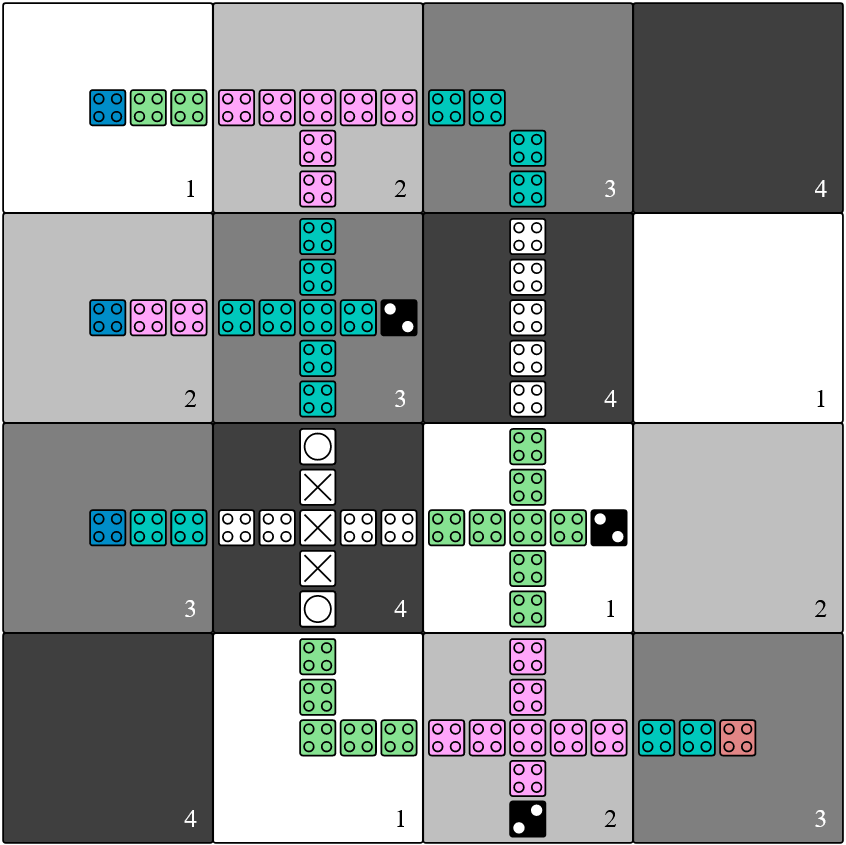
\includegraphics[scale=0.5]{input_network_mux_21}
	\caption{Placement and routing of a 2:1 mux network using the ortho algorithm with the ordering distribution network}\label{fig:input_network_mux_21}
\end{figure}

Some other issues are related to inverter nodes. Assuming an inverter node which is assigned $south$ e.g. after a fan-out node and it should be placed in the same row as an primary input, a conflict arises because the input always has to wire in x-Direction. Thus, all inverters colored $south$ need to be placed to minimum the row of the most southern primary input plus one. In order to prevent to much overhead produced by inverters a balancing network is introduced, which aims to reduce the number of inverters in the logic network. Based on the substitution of the logic network into $N$ with inverter and fan-out nodes in some cases a fan-out node has two inverters connected to its outgoing edges. Then these inverters are substituted by one single inverter as incoming node to the fan-out, resulting in an overall lower number of inverter nodes.
Figure \ref{fig:input_network_mux_21} shows the placement and routing of the ortho algorithm after implementing the proposed ordering distribution network. The ordering of the inputs puts first the fan-out node and then the two connected primary inputs. Since the inverter is part of the ordering distribution network it gets colored $east$ and allows the AND gates connected to the PIs to be colored south and the new rule for placement and routing can be applied. The last OR gate is not part of the distribution network and is therefore placed after the normal rules of the ortho algorithm. In the comparison to the layout in figure \ref{fig:ortho_mux_21} can be quickly seen that the resulting layout saves up place and even wire crossings. The exact results are presented and analyzed in the next chapter.

\section{Majority Gate Distribution Network}\label{sec:majgatedisnet}
In this section the placement and routing of majority gates, using the ortho algorithm is discussed and an accordingly distribution network is proposed. The placement and routing of majority gates plays a major role in QCA since the majority function can be implemented using only one gate in contrast to a CMOS implementation using multiple gates, following definition \ref{Def:majf}. But this theoretical advantage can only be exploited, if an efficient placement and routing exists. For this reason, in the following a majority gates distribution network for ortho is introduced, allowing the placement and routing of majority gates and therefore enabling a comparison of design metrics after placing and routing a logic network in MIG representation with its corresponding logic network in AIG representation.

\subsection{The proposed signal distribution Network}

\begin{figure}
	\centering
	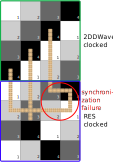
\includegraphics[scale=0.5]{Timing_failure_RES}
	\caption{Global sychronization violation when connecting 2DD-Wave and RES clocked scheme}\label{fig:Timing_failure_RES}
\end{figure}

Since the ortho algorithm uses 2DDWave clocking, the direction assignment is limited to just two options, $east$ and $south$ and the algorithm is only capable of handling the placement and routing of 2-input logic gates. Since the goal of the distribution network is to introduce "+"-majority gates into the layout a RES-like clocking needs to be utilized, introducing tiles with three incoming tiles and one outgoing tile. In the RES scheme in figure \ref{subfig:RES} such a tile is on position $(1, 1)$ and would be suited to place a "+" majority gate on it and allowing it to be connected with three incoming signals. However, simply changing the clocking scheme of ortho to RES would be really inefficient and could not be easily implemented. This is, because if the clocking would be completely changed to RES, the algorithm could not utilize every row and column of the clocking, since the RES scheme supports signals to flow into western or northern direction. Hence, in RES only the first and third row and the second and fourth column support eastern and southern signal propagation, so only these part of the clocking would be utilized for the placement of two input gates, which should lead to about a doubling in area usage considering only two-input logic gates. 
Another idea utilizing the RES scheme would be to only support it in some evenly distributed regions, supporting majority gates just at some permanently assigned places. For this the layout could be divided into $4x4$ tiles sub-regions and e.g. every fifth sub-region would be RES clocked and the rest would be occupied with the 2DDWave scheme. On the one hand, this realization should not produce as much area overhead, since only some regions are inaccessible for two input logic gates, but the permanent clocking assignment only allows the placement of majority gates gets forced on some permanent spots, leading again to large area overhead if a majority gate should be placed far away from such a sub-region. Considering a network consisting of mainly majority gates, this implementation would also waste most of the 2DD-Wave clocked area. Another aspect, which has to be taken into consideration is the trivial global synchronization constraints within a uniformly 2DDWave clocked layout, which get disrupted by introducing RES clocking within the layout. By introducing irregular clocking e.g. RES sub-regions, signals can pass a different amount of tiles in order to reach the same tile, therefore violating the global synchronization constraint. In Figure \ref{fig:Timing_failure_RES} the top four rows are 2DD-Wave clocked and the bottom four rows are RES clocked. In the 2DD-Wave scheme all three paths start globally synchronized. The two left paths need exactly one cock cycle to the majority gate. For the right path, the RES scheme causes a delay, so that the signal travels two clock cycles until reaching the majority gate, therefore violating the global synchronization constraint.

%On the other hand, for the placement of three input majority gates a new direction assignment would have to be introduced to the logic network, since one signal would need a direction assignment $west$, changing the theory and complexity underlying the ortho algorithm.

\begin{figure}
	\centering
	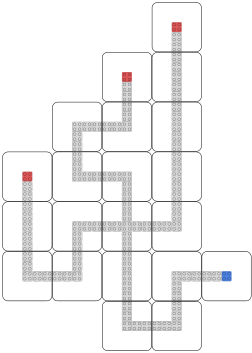
\includegraphics[scale=0.3]{Majority_Distribution_network}
	\caption{Proposed majority gate distribution network}\label{fig:QCA_Maj_nw}
\end{figure}


To avoid these complications, the proposed distribution network utilizes a custom clocking only in areas where majority gates are placed and find a solution for the global signal synchronization constraint. Therefore the placement and routing of solely two input gates should not produce any excess area. Figure \ref{fig:QCA_Maj_nw} shows the proposed majority gate signal distribution network, which is implemented into the ortho algorithm. The red marked cells indicate the three inputs for the majority gate distribution network. The cells in the middle of the tile are marked, because they can be connected from above north or the west, which would result once in a normal wire and once in a bent wire. The output in blue enables the algorithm to wire it in east or in south direction, hence allowing the algorithm to work without limitations. It is also important to mention that the input tiles as well as the output tiles have the same clocking number as in a regular 2DDWave scheme, allowing straight forward connections. Although no area overhead is produced for the already existing placement and routing of two-input gates, it can already be seen that the distribution network itself produces excess area due to its complex wiring, resulting again from the synchronization conditions that had to be considered designing it. The implementation of an AIG representation of the majority function implemented with ortho is depicted in figure !! to visualize that the placement and routing of this single majority gate barely safes area, although it has to be highlighted that no wire crossings are used. Under the assumption of really high costs for wire crossings the found majority gate distribution network is considered to be more ideal, even though a meaningful cost comparison of these two implementations can only be done under a cost function representing wire crossings in cost of normal gates.\\
In the following the design constraints used to design the signal distribution network are discussed. Firstly, the distribution network should not contain any wire-crossings, since they are considered to be very costly. Introducing a cost-metric for wire-crossings may result in a more efficient implementation, but for this work wire-crossings should be excluded as design rule for the network. Secondly, the distribution network needs to meet the global synchronization constraint. Considering a 2DDWave clocked layout, every diagonal is synchronous and every signal wired on the same diagonal passes the same amount of tiles following the ortho placement and routing. If we look at the incoming tiles of a three input tile, it can be seen that only two of the incoming tiles are on the same diagonal and the third one is shifted by half a clock cycle. Hence the third incoming signal is delayed by half a clock cycle violating the global synchronization constraint. Also the signals need to pass a multiple of whole clock cycles in the signal distribution network in order to support the further use of 2DDWave and the local synchronization constraint. Therefore, first the initially synchronous signals are also delayed by half a clocking signal, satisfying the global synchronization constraint at the tile, where the majority gate is placed. Afterwards the output signal of the majority gate is again delayed by half a clock cycle so it can be connected to the regular 2DDWave clocking scheme used in the remaining layout. Adding up the delays resulting from the distribution networks leads to a total delay of one whole clock cycle of the signal propagating through the majority gate distribution network compared to all other signals in the logic network. Because the delay affects the gloal synchronization constraint, it has to be considered for each gate connected to the parents of a majority gate distribution network. In the following first the basic placement and routing of the majority gate distribution network and then the solution for meeting the global synchronization constraint in further placement and routing is discussed. 

\subsection{Placement and routing}

\begin{figure}
	\centering
	\begin{tikzpicture}[node distance={2cm and 2cm}, thick, main/.style = {draw, rectangle}] 
		\node[fit={(0,0) (8, 8)}, inner sep=0pt, draw=black, thick] (frame) {};
		\node[fit={(1,0) (7, 8)}, inner sep=0pt, draw=black, thick, fill=lightgray] (wires) {};
		\node[fit={(1,5) (3, 8)}, inner sep=0pt, draw=black, thick, fill=cyan] (logic) {C. logic \\ w/o MAJ};
		\node[fit={(3,4) (4, 5)}, inner sep=0pt, draw=black, thick, fill=yellow] (logic) {MAJ};
		\node[fit={(4,3) (5, 4)}, inner sep=0pt, draw=black, thick, fill=cyan] (logic) {};
		\node[fit={(5,2) (6, 3)}, inner sep=0pt, draw=black, thick, fill=yellow] (logic) {MAJ};
		\node[fit={(6,0) (7, 2)}, inner sep=0pt, draw=black, thick, fill=cyan] (logic) {};
		
		\node[fit={(0,6.5) (1, 8)}, inner sep=0pt, draw=black, thick, fill=TUMGray] (PIs) {PIs};
		\node[fit={(7,0) (8, 8)}, inner sep=0pt, draw=black, thick, fill=TUMGray] (POs) {POs};
		
		
		
		\draw (3.5,1) node [align = left] {Area for wiring \\ and buffer insertion};
		
		
	\end{tikzpicture} 
	\caption{Scheme of the P\&R using the Majority Gate Distribution Network} \label{fig:majority_scheme}
\end{figure}

The placement and routing of the proposed signal distribution network is again bound to some constraints. First of all the coloring of majority gates has to be reviewed, since the logic network now includes three input nodes. However, the coloring algorithm can include helping nodes to resolve coloring conflicts of edges and therefore dividing every edge with a helping node shows, that a trivial coloring can be found also including three input nodes into the logic network. Another aspect regarding coloring is the need for a new direction in order to connect a third signal to the majority gate, but since the only occasion such a wiring happens is inside the fixed distribution network, which again can be placed and routed in the usual south-eastern manner, no additional directions need to be included. Further, the irregular clocking inside the signal distribution network has to be reviewed. These irregularities don't allow the algorithm to wire connections over the network, demanding a special treatment for the placement of the majority gates. From the algorithms perspective therefore a majority gate cannot be placed just south or east of another gate because these gates could need a wiring through the majority gate distribution network. Instead the algorithm is forced to assign the majority gate distribution network always south \textbf{and} east direction to prevent routing conflicts. This means that for majority gates always a trivial coloring is chosen. The major drawback of this is, that again the area is not used optimally and the layout is extended in two directions as shown in figure \ref{fig:majority_scheme} compromising the beneficial use of the "+"-majority gate.

\subsection{Signal synchronization and buffer insertion}
The placement and routing using the proposed distribution network results in a delay of one clock cycles of signals passing through a majority gates. Since the tile-based clocking doesn't support a speedup of a signal, every other signal which comes into contact with a delayed signal also has to be delayed in order to meet the global synchronization constraint. Therefore a function is introduced to compute the delay of signals and allowing signals which are connected together to be synchronized by buffer insertion. For the delay computation, the algorithms views every incoming edge from every node starting at the primary output. If an incoming edge is connected to a majority gate, every other incoming edge of the same node gets a delay of one assigned, if this edge is not also connected to a majority gate. In the latter case all incoming edges of a node are delayed, resulting again in synchronous behavior. Nodes with incoming edges from majority gates are marked as delayed and the delays stack for every majority gate on a path. The inserted delays then result from the difference of delays of the incoming edges from a node and are realized by inserting wire buffers. 

\begin{figure}
	\centering
	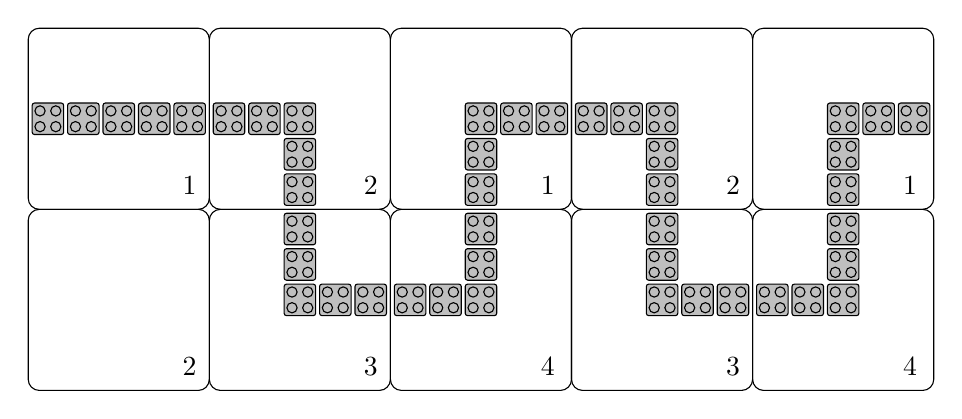
\begin{tikzpicture}
		\begin{scope}[xshift=-2.3cm, rotate=90]
			\draw[rounded corners] (-0.05, -0.1 - 0.85) rectangle (2.3-0.05, 2.3-0.1 - 0.85){};
			
			\foreach \x/\y in {0.9/0.9, 0.9/0.45, 0.9/0, 0.9/-0.45, 0.9/-0.9}
			{
				\draw[rounded corners = 0.3mm, fill=lightgray] (\x, 0 + \y) rectangle (1.2/3 + \x, 1.2/3 + \y){};
				\draw (0.3/3+ \x,0.3/3 + \y) circle (0.65mm);
				\draw (0.9/3+ \x,0.3/3+ \y) circle (0.65mm);
				\draw (0.3/3+ \x,0.9/3 + \y) circle (0.65mm);
				\draw (0.9/3+ \x,0.9/3 + \y) circle (0.65mm);
			}
			\node[text=black] (A1) at (0.25,-0.7) {$1$};
		\end{scope}
		\begin{scope}[xshift=-2.3cm, yshift=-2.3cm, rotate=90]
			\draw[rounded corners] (-0.05, -0.1 - 0.85) rectangle (2.3-0.05, 2.3-0.1 - 0.85){};
			
			\node[text=black] (A1) at (0.25,-0.7) {$2$};
		\end{scope}
		\begin{scope}[shift={(0, 0)}, rotate=90]
			\draw[rounded corners] (-0.05, -0.1 - 0.85) rectangle (2.3-0.05, 2.3-0.1 - 0.85){};
			
			\foreach \x/\y in {0.9/0.9, 0.9/0.45, 0.9/0, 0/0, 0.45/0}
			{
				\draw[rounded corners = 0.3mm, fill=lightgray] (\x, 0 + \y) rectangle (1.2/3 + \x, 1.2/3 + \y){};
				\draw (0.3/3+ \x,0.3/3 + \y) circle (0.65mm);
				\draw (0.9/3+ \x,0.3/3+ \y) circle (0.65mm);
				\draw (0.3/3+ \x,0.9/3 + \y) circle (0.65mm);
				\draw (0.9/3+ \x,0.9/3 + \y) circle (0.65mm);
			}
			\node[text=black] (A1) at (0.25,-0.7) {$2$};
		\end{scope}
		\begin{scope}[xshift=3.2cm, yshift=1.3cm, rotate=180]
			\draw[rounded corners] (-0.05, -0.1 - 0.85) rectangle (2.3-0.05, 2.3-0.1 - 0.85){};
			
			\foreach \x/\y in {0.9/0.9, 0.9/0.45, 0.9/0, 0/0, 0.45/0}
			{
				\draw[rounded corners = 0.3mm, fill=lightgray] (\x, 0 + \y) rectangle (1.2/3 + \x, 1.2/3 + \y){};
				\draw (0.3/3+ \x,0.3/3 + \y) circle (0.65mm);
				\draw (0.9/3+ \x,0.3/3+ \y) circle (0.65mm);
				\draw (0.3/3+ \x,0.9/3 + \y) circle (0.65mm);
				\draw (0.9/3+ \x,0.9/3 + \y) circle (0.65mm);
			}
			\node[text=black] (four) at (0.25 ,1.05) {$1$};
		\end{scope}
		\begin{scope}[xshift=-0.4cm, yshift=-0.1cm, rotate=270]
			\draw[rounded corners] (-0.05, -0.1 - 0.85) rectangle (2.3-0.05, 2.3-0.1 - 0.85){};
			
			\foreach \x/\y in {0.9/0.9, 0.9/0.45, 0.9/0, 0/0, 0.45/0}
			{
				\draw[rounded corners = 0.3mm, fill=lightgray] (\x, 0 + \y) rectangle (1.2/3 + \x, 1.2/3 + \y){};
				\draw (0.3/3+ \x,0.3/3 + \y) circle (0.65mm);
				\draw (0.9/3+ \x,0.3/3+ \y) circle (0.65mm);
				\draw (0.3/3+ \x,0.9/3 + \y) circle (0.65mm);
				\draw (0.9/3+ \x,0.9/3 + \y) circle (0.65mm);
			}
			\node[text=black] (A1) at (1.1+0.85,1.1) {$3$};
		\end{scope}
		\begin{scope}[xshift=1cm, yshift=-1.4cm, rotate=0]
			\draw[rounded corners] (-0.05, -0.1 - 0.85) rectangle (2.3-0.05, 2.3-0.1 - 0.85){};
			
			\foreach \x/\y in {0.9/0.9, 0.9/0.45, 0.9/0, 0/0, 0.45/0}
			{
				\draw[rounded corners = 0.3mm, fill=lightgray] (\x, 0 + \y) rectangle (1.2/3 + \x, 1.2/3 + \y){};
				\draw (0.3/3+ \x,0.3/3 + \y) circle (0.65mm);
				\draw (0.9/3+ \x,0.3/3+ \y) circle (0.65mm);
				\draw (0.3/3+ \x,0.9/3 + \y) circle (0.65mm);
				\draw (0.9/3+ \x,0.9/3 + \y) circle (0.65mm);
			}
			\node[text=black] (four) at (1.95 ,-0.65) {$4$};
		\end{scope}
		
		\begin{scope}[xshift=4.6cm, yshift=0cm, rotate=90]
			\draw[rounded corners] (-0.05, -0.1 - 0.85) rectangle (2.3-0.05, 2.3-0.1 - 0.85){};
			
			\foreach \x/\y in {0.9/0.9, 0.9/0.45, 0.9/0, 0/0, 0.45/0}
			{
				\draw[rounded corners = 0.3mm, fill=lightgray] (\x, 0 + \y) rectangle (1.2/3 + \x, 1.2/3 + \y){};
				\draw (0.3/3+ \x,0.3/3 + \y) circle (0.65mm);
				\draw (0.9/3+ \x,0.3/3+ \y) circle (0.65mm);
				\draw (0.3/3+ \x,0.9/3 + \y) circle (0.65mm);
				\draw (0.9/3+ \x,0.9/3 + \y) circle (0.65mm);
			}
			\node[text=black] (A1) at (0.25,-0.7) {$2$};
		\end{scope}
		\begin{scope}[xshift=7.8cm, yshift=1.3cm, rotate=180]
			\draw[rounded corners] (-0.05, -0.1 - 0.85) rectangle (2.3-0.05, 2.3-0.1 - 0.85){};
			
			\foreach \x/\y in {0.9/0.9, 0.9/0.45, 0.9/0, 0/0, 0.45/0}
			{
				\draw[rounded corners = 0.3mm, fill=lightgray] (\x, 0 + \y) rectangle (1.2/3 + \x, 1.2/3 + \y){};
				\draw (0.3/3+ \x,0.3/3 + \y) circle (0.65mm);
				\draw (0.9/3+ \x,0.3/3+ \y) circle (0.65mm);
				\draw (0.3/3+ \x,0.9/3 + \y) circle (0.65mm);
				\draw (0.9/3+ \x,0.9/3 + \y) circle (0.65mm);
			}
			\node[text=black] (four) at (0.25 ,1.05) {$1$};
		\end{scope}
		\begin{scope}[xshift=4.2cm, yshift=-0.1cm, rotate=270]
			\draw[rounded corners] (-0.05, -0.1 - 0.85) rectangle (2.3-0.05, 2.3-0.1 - 0.85){};
			
			\foreach \x/\y in {0.9/0.9, 0.9/0.45, 0.9/0, 0/0, 0.45/0}
			{
				\draw[rounded corners = 0.3mm, fill=lightgray] (\x, 0 + \y) rectangle (1.2/3 + \x, 1.2/3 + \y){};
				\draw (0.3/3+ \x,0.3/3 + \y) circle (0.65mm);
				\draw (0.9/3+ \x,0.3/3+ \y) circle (0.65mm);
				\draw (0.3/3+ \x,0.9/3 + \y) circle (0.65mm);
				\draw (0.9/3+ \x,0.9/3 + \y) circle (0.65mm);
			}
			\node[text=black] (A1) at (1.1+0.85,1.1) {$3$};
		\end{scope}
		\begin{scope}[xshift=5.6cm, yshift=-1.4cm, rotate=0]
			\draw[rounded corners] (-0.05, -0.1 - 0.85) rectangle (2.3-0.05, 2.3-0.1 - 0.85){};
			
			\foreach \x/\y in {0.9/0.9, 0.9/0.45, 0.9/0, 0/0, 0.45/0}
			{
				\draw[rounded corners = 0.3mm, fill=lightgray] (\x, 0 + \y) rectangle (1.2/3 + \x, 1.2/3 + \y){};
				\draw (0.3/3+ \x,0.3/3 + \y) circle (0.65mm);
				\draw (0.9/3+ \x,0.3/3+ \y) circle (0.65mm);
				\draw (0.3/3+ \x,0.9/3 + \y) circle (0.65mm);
				\draw (0.9/3+ \x,0.9/3 + \y) circle (0.65mm);
			}
			\node[text=black] (four) at (1.95 ,-0.65) {$4$};
		\end{scope}
		
	\end{tikzpicture}
	\caption{Buffer in $east$ direction with resolve column and respective clocking}\label{fig:QCA_buf}
\end{figure}

Figure \ref{fig:QCA_buf} depicts a buffer in the east direction, which can also be used in the south direction by just rotating it 90 degrees. The snake-shaped structure delays a signal by exactly one clock cycle and is also used in custom placement and routing resulting from the QCA ONE library \cite{QCA_scl}. As in the majority gate distribution network, the buffers support irregular clocking, creating zones through which the algorithm cannot wire. In the case of buffers only one column or row is made impassable, allowing them to be tracked and introducing a rewiring for conflicts. Algorithm \ref{alg:majority_network} shows the code snippets which are changed and added to ortho in order to allow the placement and routing of majority gates distribution networks and the corresponding majority buffers. Figure \ref{fig:majority_with_buf} shows the placement of a majority gate inside the input distribution network and two and gates that have to be delayed to be connected to the delayed signal coming out of the majority gate distribution network. The insertion of the first buffer blocks the eastern direction of the second input. For this case, a resolve column is introduced where the signal can be assigned to a new row and be wired without conflict. From this layout, it can already be seen that the implementation of the majority gate distribution network brings several complications with it, all resulting in area overhead, which stands in contrast to the area which should be saved by introducing majority gates in the first place.

\begin{algorithm}[H]
	\vdots
	
	\begin{algorithmic}
		\State Convert $N$ to a 3-graph by substitution and balance inverters at fan-out nodes, except for majority gates
		\State Compute the delay as majority buffer insertion $buf_{maj}$ for every node and assign it to the incoming signals $\sigma$
		\State Order primary input nodes
		\State Create vectors with from the majority buffers blocked columns $bl_c$ and rows $bl_r$
		\State \vdots
		\ForAll {vertex $v_1, ..., v_i \in N $ with at most three incoming signals $\sigma_1, \sigma_2, \sigma_3$}
		\State Rewire incoming signals which are wired on $bl_c$ or $bl_r$
		\State \vdots
		\If{vertex $v$ has fanin of three (is a majority gate)}
		\If{$d(\sigma_1) = d(\sigma_2) = d(\sigma_3) = south$}
		\State{Extend $L$ by one row and wire the incoming signal to $(w_p, h-1)$ for every incoming signal}
		\EndIf
		\State Insert majority buffers according to the delay computed in $buf_{maj}$ and safe blocked columns $bl_c$ and rows $bl_r$
		\State Extend the layout by number of rows $(7)$ and columns $(5)$ of the majority gate distribution network and place the distribution network at $(w-5, h-7)$
		\State Connect incoming signals west to the inputs of the distribution network
		\ElsIf{$d(\sigma_1) = d(\sigma_2) = east$}
		\State Insert majority buffers according to the delay computed in $buf_{maj}$ and safe blocked rows $bl_r$
		\State \vdots
		\ElsIf { signals are labeled $south$}
		\State Insert majority buffers according to the delay computed in $buf_{maj}$ and safe blocked columns $bl_c$
		\State \vdots
		\EndIf
		
		\EndFor
%		\State \vdots \\
%		\Return $L$
	\end{algorithmic}
	\caption{Ortho changes with majority gate distribution network}\label{alg:majority_network}
\end{algorithm}

\begin{sidewaysfigure}
	\centering
	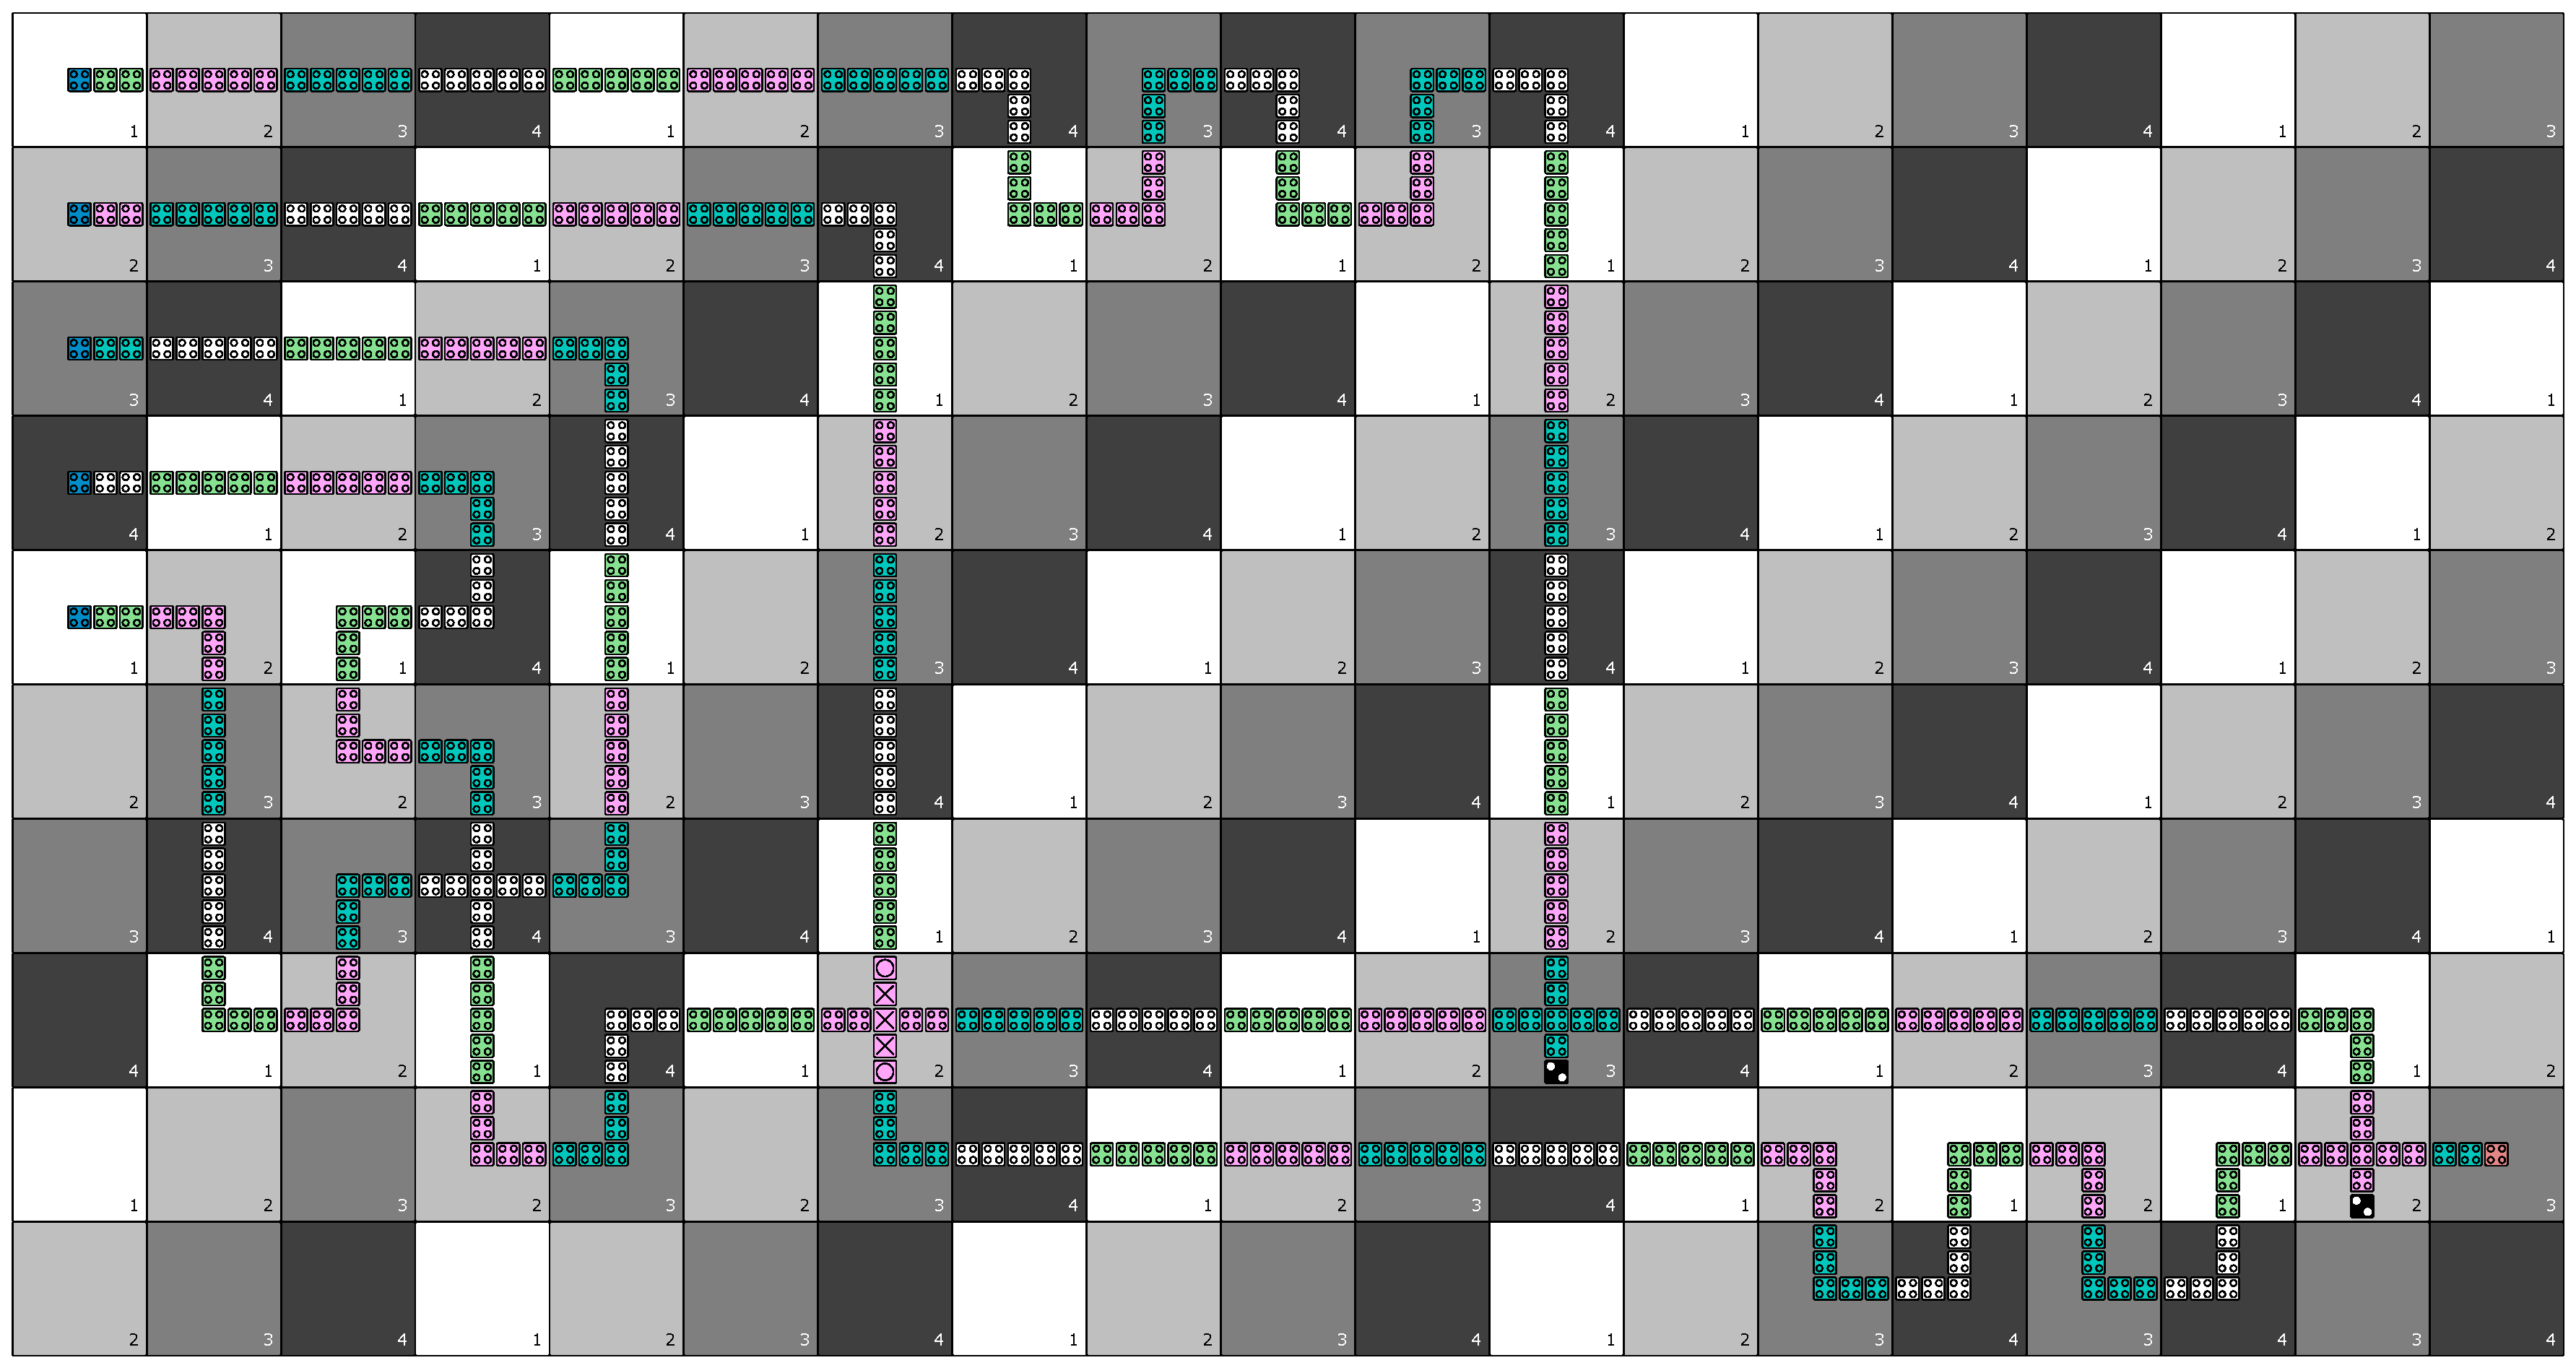
\includegraphics[scale=0.33]{TEST_maj_two_buf_cell_lvl_lyt_2}
	\caption{Placement and routing of a majority distribution network in conjunction with two primary inputs}\label{fig:majority_with_buf}
\end{sidewaysfigure}


\section{Sequential Distribution Network}
In this section, a distribution network is provided, which enables ortho to automatically design sequential circuits. To the authors' knowledge, there has been no solution to place and route sequential circuits in QCA yet. The only algorithms dealing with sequentiality in QCA, presented in Chapter \ref{chapter:SotA}, only translate CMOS structures directly into QCA and therefore require an external clock signal, which was stated to be unnatural, because QCA has its own clocking paradigm. For the placement and routing used here, the ideas of gates, able to delay signals from \cite{Walter}, was used and further developed for the automated placement and routing.

\subsection{Placement and Routing}
Before looking at the algorithm, first the idea of an FF wire should be discussed in the domain of placement and routing and not only as a single element. From the FF wire it can be examined that the proposed FF implementation requires more complex clock generators for every FF, and it is not sure if this is possible to implement. Also if we look back at the analogy of CMOS, a sequential circuit includes a combinational logic block and the storage element, which is formed by a wire FF in this case. But there is still a big difference. While in CMOS the information can just be arbitrarily wired back from the storage to the inputs of the combinational logic, in QCA the wiring back implies the placement of wire segments of which each is delaying the information by one clocking zone already, being a partial FF. If a signal is wired through four adjacent wire gates, a basic FF is already formed, since the information is delayed by four clock zones equaling a clock cycle. When looking back to the functionality of a storage element, it can be found that this delay is exactly the purpose of a clocking element and the reason why the clocking for the wire FF is customized. The idea proposed in this work is now to use the delay, which occurs naturally due to sequential wiring to mimic storage elements and therefore wire segments can be summarized to FFs without the need for customized clocking. 

\begin{figure}
	\centering
	\begin{tikzpicture}[node distance={2cm and 2cm}, thick, main/.style = {draw, rectangle}] 
		\node[fit={(0,0) (8, 8)}, inner sep=0pt, draw=black, thick] (frame) {};
		\node[fit={(2,2) (6, 8)}, inner sep=0pt, draw=black, thick, fill=cyan] (logic) {Combinational logic};
		\node[fit={(0,6.5) (1, 8)}, inner sep=0pt, draw=black, thick, fill=TUMGray] (PIs) {PIs};
		\node[pattern=north west lines, pattern color=TUMGray, fit={(1,6.5) (2, 8)}, inner sep=0pt, draw=black, thick] (wires) {wires};
		\node[fit={(1,5) (2, 6.5)}, inner sep=0pt, draw=black, thick, fill=lightgray] (ROs) {ROs};
		\node[pattern=north west lines, pattern color=TUMGray,fit={(6,3.5) (7, 8)}, inner sep=0pt, draw=black, thick] (wires) {wires};
		\node[fit={(7,3.5) (8, 8)}, inner sep=0pt, draw=black, thick, fill=TUMGray] (POs) {POs};
		\node[fit={(6,2) (7, 3.5)}, inner sep=0pt, draw=black, thick, fill=lightgray] (RIs) {RIs};
		
		\draw[] (7, 3.5) -- (8, 3.5);
		\draw[] (0, 6.5) -- (1, 6.5);
		\draw[fill=Apricot] (0, 0) -- (0, 6.5) -- (1, 6.5)  -- (1, 5) -- (2, 5) -- (2, 2) -- (7, 2) -- (7, 3.5) -- (8, 3.5) -- (8, 0) -- (0, 0);
		\draw (4,1) node [align=left] {Sequential wires from Ris to Ros \\ with delay of $c$ clock cycles};
		%		\draw[->] (2) -- (5);
		%		\draw[->] (3) -- (6);
		%		\draw[->] (4) -- (6);
		%		\draw[->] (5) -- (7);
		%		\draw[->] (6) -- (7);
		%		\draw[->] (7) -- (f);
		
	\end{tikzpicture} 
	\caption{Scheme of a sequential circuit layout after placement and routing} \label{fig:sequential_gate_sample}
\end{figure}

Considering the placement and routing of sequential circuits, not only a distribution network has to be designed but also the logic network has to be expanded regarding to storage elements. They are represented in the logic network by registers with its corresponding input, determining the value, which has to be stored, and its output, which gives the register value to the combinational logic again after delaying it to the next \textit{circuit clocking cycle}. A circuit clocking cycle refers to one cycle of Bennet clocking that has propagated through the circuit completely. The registers are implemented into the logic network as follows. Register inputs (RIs) are treated similar to primary outputs, therefore they are dangling edges, which point to no node but additionally have a register output assigned. Register outputs (ROs) are treated similarly to primary inputs, being terminal vertices, but always feeding in the data which were given to the corresponding register input in the last circuit clocking cycle. Therefore, the logic network extends to $N = (\Lambda, I, RO, \Sigma, O, RI)$. Here it has to be mentioned that for the input distribution network due to their similarity ROs can be treated just like PIs, enabling the combination with the sequential distribution network.
Also, for placement and routing, the similarities between PIs/ROs and POs/RIs can be exploited. The schematic layout resulting from the described algorithm is shown in figure \ref{fig:sequential_gate_sample}. When the first part of ortho is performed, first the combinational logic part is placed and routed, treating ROs just like PIs and RIs just like POs. From this stage, a routing from the RIs to the ROs has to be found, which retains the local and global synchronization constraint. Because every register input has exactly one register output assigned, first of all, the register inputs are rewired and sorted in the same order as the register outputs. The ordering follows in a way that all RIs are put on a diagonal, and since to this point every gate is clocked uniformly with 2DDWave, the signals are all synchronized. With this starting position now wires with the same length have to be found between every register input and output. Since the wires now also have to go in western and northern directions in order to close the loop between the ROs in the upper left corner and the RIs in the down-right corner of the layout, the wiring is not arbitrary. One big issue is also that the clocking cannot be chosen independently for each back-loop because the loops cross each other. The solution found can be seen in an example depicted in figure !!. From this example another issue regarding timing can be derived. Considering a primary Input in a completely combinational circuit being placed in the fifth row of the layout. In this case the PI is set in a different \textit{time zone}, because its signal is globally delayed by one clock cycle. Until now the assumption was made, that an input network can be used to delay the primary input by one clocking cycle to achieve again global synchronization. When an RO is placed in a different time zone, this also has to be respected by the wiring of the registers. As already mentioned, the registers do not delay the information by only one clocking cycle but by multiple clocking slowing down the performance of the circuit drastically. This huge delay is due to the fact that ortho lays the combinational logic only in the south-eastern direction, always increasing the distance between PIs/ROs and POs/RIs. Therefore the sequential signal distribution network always grows with the size of the combinational logic.\\
Maybe a folding operation can be found for the ortho algorithm so that the distance between RIs and ROs can be decreased and therefore the delay produced by the sequential distribution network can be decreased as well.

\subsection{RAM cell}
As mentioned in \ref{subsec:RAM_SoA}, a RAM cell can be realized using wire delays to safe the data and a MUX, which can input new data into the RAM cell. With the possibility of placing and routing sequential circuits a RAM cell now is a MUX with two PIs and one RO. The PIs are the BL and WL, while the RO is the information held in the RAM cell. The output of the MUX is both the PO and the RI.
Figure \ref{fig:QCA_RAM} shows a RAM cell, with its respective wordline(s), bitline(s) and latch. The core of the cell is a latch, which is simply propagating the data in a circle and therefore producing a stable output once in every clock cycle. The input mechanism works via two majority gates. The majority gates with the wordlines decides if $BL$ or $\bar{BL}$ should be propagated to the majority gate connected to the loop. When $WL_1=\bar{WL_2}$ the majority gate always outputs the third input $BL$. But for $WL_1=WL_2=\bar{BL}$ the first majority gate outputs $\bar{BL}$.
If the first majority gate has as output $BL$, the second majority gate has $BL$ twice as input and overrides the data in the RAM cell. If the first majority gate has as output $\bar{BL}$, the second majority gate has two distinct inputs and the data which is held in the cell. In this case the stored bit always decides the output and therefore it is latched meaning that the data is stored. For the read operation only one majority gate is needed and in order to read the RAM cell the output-wordlines have to be inverted. Otherwise if both output-worlines are set to "0", the output isn't read. The corresponding truth tables for the RAM cell is shown in \ref{subfig:QCA_RAM_tt}.
\begin{figure}
	\centering
	\subfigure[QCA implementation]
	{
		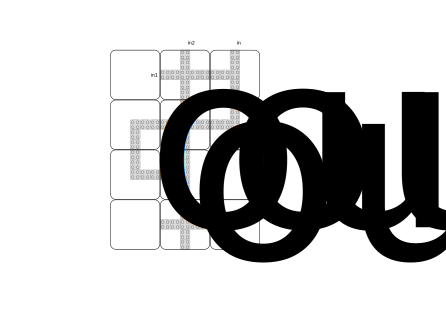
\includegraphics[scale=0.4]{RAM_cell}
	}
	\subfigure[Truth table]
	{
		% Table generated by Excel2LaTeX from sheet 'Tabelle1'
		\centering
		\begin{tabular}{cllll}
			& Input1 & Input2 & Input3 & Output \\
			\multirow{2}[0]{*}{Maj1} & $WL_1$   & $WL_2=\overline{WL_1}$ & $BL$    & $BL$ \\
			& $WL_1=\overline{BL}$ & $WL_2=\overline{BL}$ & $BL$    & $\overline{BL}$ \\
			\multirow{2}[0]{*}{Maj2} & $X$     & $BL$    & $BL$    & $BL$ \\
			& $X$     & $\overline{BL}$ & $BL$    & $X$ \\
		\end{tabular}%
		\label{subfig:QCA_RAM_tt}
	}
	\caption{QCA RAM cell using wire delay}\label{fig:QCA_RAM}
\end{figure}